\section{Derivation of the analytic posterior for toy example}
\label{sec:analytical_posterior}

In this appendix we derive and compute the conditional distribution \(\Fcond\) for the toy example of \autoref{sec:toy_example}.
We denote by \(f_i(\cdot)\) and \(F_i(\cdot)\) the prior probability distribution function and cumulative distribution function of \(X_i\), i.e. the normal PDF and CDF with means and variances given by \autoref{eq:toyspec}.
Let \(\pij\) be the probability that \(X_i\) is the minimum of \(X\) and \(X_j\) is its maximum.
We also define \(\pisum = \sum_{j=1}^{100} \pij\), the probability that \(X_i\) is the minimum,
and \(\psumj = \sum_{i=1}^{100} \pij\), the probability that \(X_j\) is the maximum.
The cumulative distribution function of \(X_i\) is then given by:
\begin{equation}
\Pr\del{X_i \leq x \mid \Xmax, \Xmin} =
    \begin{cases}
        0 &\text{if } x < \Xmin \,, \\
        1 &\text{if } x \geq \Xmax \,, \\
        \pxx{i}{\bullet} 
            + \del{1 \!-\! \pxx{i}{\bullet} \!-\! \pxx{\bullet}{i}}
            \sbr{\frac{F_i(x) - F_i(\Xmin) }
                 {F_i(\Xmax) - F_i(\Xmin) }
                } 
            &\text{otherwise.}\\
    \end{cases}
\end{equation}
Meanwhile, \(\pij\) is proportional to:
\begin{equation}
    f_i(\Xmin)
    f_j(\Xmax)
    \prod_{k \neq i,j}^{100}
    \del{F_k(\Xmax) - F_k(\Xmin)} \,,
\end{equation}
which we compute for all \(i,j\) and normalize
to obtain the \(100 \times 100\) matrix \(\Pr\) of probabilities of each pair of element occupying the extremes.
We sum over its rows and columns to obtain \(\psumj\) and \(\pisum\).
While this algorithm has cubic complexity in the dimensionality \(p\) of \(X\),
for \(p=100\), it only take seconds to compute the entries of \(\Pr\) and evaluate \(\Pr\del{X_i \leq x \mid \Xmax, \Xmin}\) over a range of \(x\).
\autoref{fig:toy_quantiles}(b) shows the analytical quantiles of \(\Fcond\) marginally for each \(X_i\).

\section{Modeling the diurnal cycle with Gaussian processes}
\label{appendix:diurnal_kernel}

Reviewers of earlier versions of this paper have raised concerns about our use of a periodic kernel,
instead of a periodic mean function in \autoref{eq:kdiurn} and \autoref{eq:sumprod_kernel}.
It is indeed commonplace in geostatistics to specify a mean functions that is the sum of harmonics
with a period of 24 hours (diurnal cycle) or 365 days (seasonal cycle) and integer fractions thereof:
\begin{equation}
    m(t) = \sum_{w=1}^W \sbr{a_w \cos(2\pi t w / 24) + b_w \sin(2\pi t w / 24)}
    \label{eq:mperiodic}
\end{equation}
with $W$ typically chosen to be between 1 and 5, and coefficients fitted by maximizing the marginal likelihood.
For example, this is the approach taken (with $W=1$) to model the seasonal component in a closely related application by \citet{kleiber2013daily}.
Since the mean function is frequently interpreted as capturing long-term trends (climate component), while the Gaussian process captures stochastic deviations from the trend (weather component), it is perceived as a natural choice to incorporate periodic components in the mean function.
However common, this narrative clashes with a Bayesian understanding of the Gaussian process.
Rather than optimizing the ($a_w,b_w$) coefficients, a Bayesian would generally prefer to equip them with priors,
and propagate their uncertainty to inferences and predictions.
A relatively uncontroversial choice would be an independent normal prior $\normal(0, \sigma^2)$ on each coefficient, 
but then it is noticed that this induces a covariance between $m(t)$ and $m(t')$ of 
$\sigma^2 \sum_{w=1}^W 
        \sbr{
            \cos(2\pi t w / 24) \cos(2\pi t' w / 24) + 
            \sin(2\pi t w / 24) \sin(2\pi t' w / 24)
            }$.
The resulting model is therefore strictly mathematically equivalent to a Gaussian process
with such a term added to the covariance kernel.
The only difference between this augmented $\GP$ 
and the mean function specification \autoref{eq:mperiodic} is that the 
uncertainty in the coefficients is now rigorously accounted for.
This reasoning holds for any linear basic function in the mean.

But rather than using this kernel derived from a finite sine and cosine basis,
we have opted to use the periodic kernel \autoref{eq:kperiodic},
which has the significant advantage of being able to fit any continuous periodic function
with only two hyperparameters (we hold the period fixed of course).
We now illustrate this advantage with a simulation from the model:
\begin{equation}
\begin{split}
    v_{24}(t) &= 5 \log\sbr{ \cos(2\pi t / 24) + 1.02} \text{, the diurnal cycle,}\\
    f(t) & \sim \GP(v_{24}(t), k(t,t')) \text{, the process,}\\
    y_i &= f(t_i) + \epsilon_i, \quad \epsilon_i \sim \normal(0, 0.1^2) \text{, the observations, }
\end{split}
\end{equation}
where time $t$ is in hours, and the $\GP$ kernel is Mat\'ern 3/2 with lengthscale 0.5 hours and variance parameter $(1.5)^2$.
We simulate 7 days of data, but withhold data from the fifth day (\autoref{fig:periodic_sim}).
We then fit the following 5 Gaussian process models:
\begin{enumerate}
    \item A constant plus periodic mean function with $W=2$ and the Mat\'ern 3/2  kernel;
    \item A constant plus periodic mean function with $W=4$ and the Mat\'ern 3/2  kernel;
    \item A constant plus periodic mean function with $W=6$ and the Mat\'ern 3/2  kernel;
    \item A constant mean function with a sum kernel of Mat\'ern 3/2 plus periodic \autoref{eq:kperiodic}.
    \item A constant plus periodic mean function with $W=2$ and a sum kernel of Mat\'ern 3/2 plus periodic.
\end{enumerate}
Each model is initialized with all mean parameters set to zero, and the Mat\'ern coefficients set to their true value,
while the periodic kernel is initialized with $\ell=1$ and variance $1$.
We then optimize the parameters and obtain predictions for the fifth day, which are shown in \autoref{fig:periodic_results}.
The resulting predictions show that the periodic kernel gives the best predictions, as the kernel was able to tightly fit the diurnal component.
The choice $W=4$ also gives good predictions, but underspecifying ($W=2$) or overspecifying ($W=6$) the mean functions leads to degraded performance.
With additional days of data, the periodic kernel will be able to fit the diurnal cycle arbitrarily well,
without necessitating additional hyperparameters.
The combination of a periodic mean function and periodic kernel does not lead to noticeably better predictions.

\begin{figure}
    \centering
    \begin{subfigure}[t]{0.32\textwidth}
    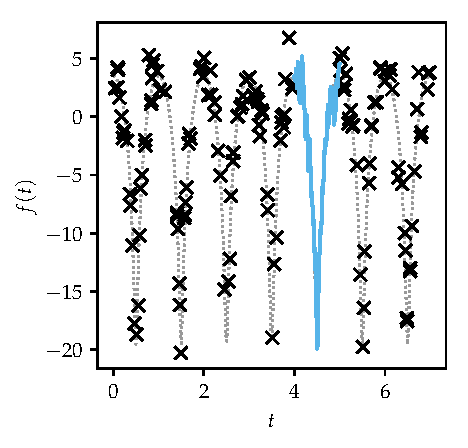
\includegraphics[width=\textwidth]{periodic/periodic_sim.pdf}
    \caption{Simulation setting}
    \label{fig:periodic_sim}
    \end{subfigure}
    \begin{subfigure}[t]{0.32\textwidth}
    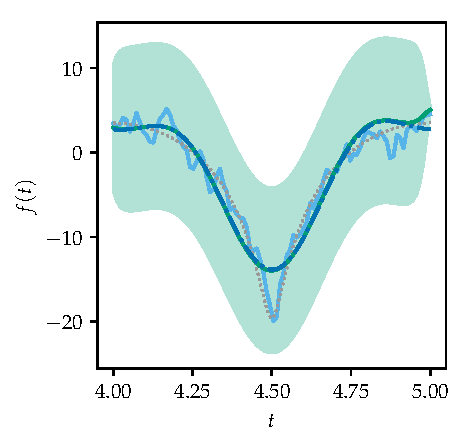
\includegraphics[width=\textwidth]{periodic/periodic_results_under.pdf}
    \caption{Periodic $m$ with $W=2$}
    \label{fig:periodic_results_under}
    \end{subfigure}
    \begin{subfigure}[t]{0.32\textwidth}
    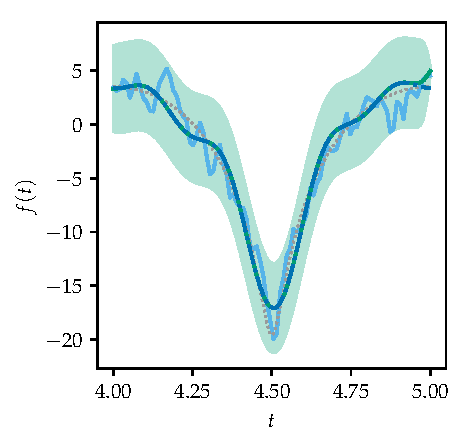
\includegraphics[width=\textwidth]{periodic/periodic_results_meanper.pdf}
    \caption{Periodic $m$ with $W=4$}
    \label{fig:periodic_results_meanper}
    \end{subfigure}
    \begin{subfigure}[t]{0.32\textwidth}
    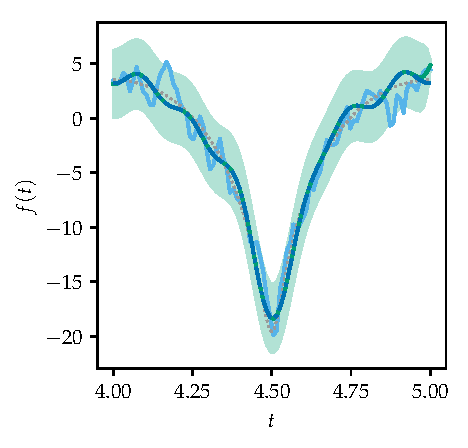
\includegraphics[width=\textwidth]{periodic/periodic_results_over.pdf}
    \caption{Periodic $m$ with $W=6$}
    \label{fig:periodic_results_over}
    \end{subfigure}
    \begin{subfigure}[t]{0.32\textwidth}
    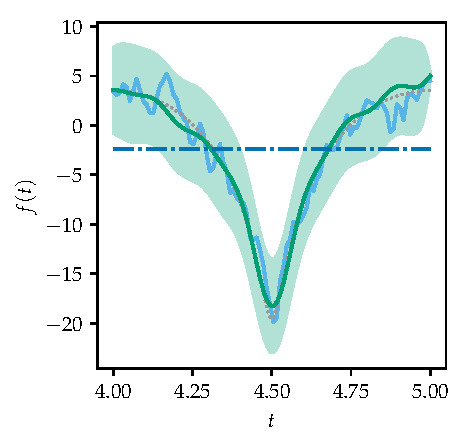
\includegraphics[width=\textwidth]{periodic/periodic_results_kper.pdf}
    \caption{Constant $m$ and periodic $k$}
    \label{fig:periodic_results_kper}
    \end{subfigure}
    \begin{subfigure}[t]{0.32\textwidth}
    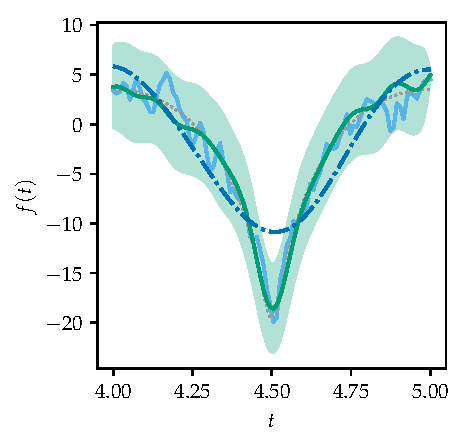
\includegraphics[width=\textwidth]{periodic/periodic_results_both.pdf}
    \caption{Periodic $m$ and periodic $k$}
    \label{fig:periodic_results_both}
    \end{subfigure}
\caption{\label{fig:periodic_results}
    Simulations comparing periodic mean functions and kernels.
    \autoref{fig:periodic_results_under} shows the observations (crosses), diurnal cycle (dotted),
    and true process in the test window (solid line).
    For each model, we show posterior mean and credible envelope (2 standard deviations),
    and the fitted mean function (dash-dotted, which often overlaps with the posterior mean).
}
\end{figure}

As an additional benefit of modeling periodic components in the kernel rather than the mean function is that drifts in the cycle (for example due to seasonal changes)
can be captured by multipling the periodic kernel with a stationary temporal kernel.
Equally, slight differences in the diurnal cycle between sites can be captured by multiplying it with a stationary spatial kernel.

\section{Technical details of batch computations}
\label{appendix:batch_details}

Because of the high computational cost of fitting GPs with many observations,
there is a large literature on sparse approximations to speed up
covariance computations \citep{quinonero2007approximation, banerjee2008gaussian, banerjee2014hierarchical},
as well as Bayesian approximation techniques such as variational Bayes \citep{beal2003variational,jordan1999introduction,ren2011variational} and the integrated nested Laplace approximation \citep{rue2009approximate}.
Each approximation makes different compromises which need careful consideration.
In particular, some techniques yield poor approximations of the posterior uncertainty,
which is crucial for our application.
For this reason, we opted for the more primitive method of processing the data
in batches: cutting the time series and fitting the full GP
model to each batch separately.
The tradeoff is explicit: we fit the full GP locally, but discard information between
measurements that are distant in time.

We argue that this is a good approximation for the present application, except at the boundaries
between batches.
For this reason, we allow some overlap between batches when obtaining predictions,
so that every prediction is made far away from these boundaries.
The duration of each batch compromises computational efficiency and the amount of information made
available to each window.
In our implementation, we used the following batch durations at each stage of the imputation strategy, referring to \autoref{fig:paper_in_one_figure}:
\begin{enumerate}[label=(\alph*),start=2]
    \item To fit the hyperparameters, we use non-overlapping 10-day windows to maximize the marginal likelihood,
          and 8-day windows to maximize the cross-validation critertion \autoref{eq:cv_criterion}, which
          is more expensive to compute.
          Within the optimization routine, we sum the objective and its gradient across batches.
          \label{step:hyperparameters}
    \item When generating predictions from the Gaussian process, only a single Cholesky decomposition
          is required, so we divide the year of data into 5 equal batches (73 days), with each
          subsequent batch starting a third of the batch duration after the start of the last one.
          \label{step:nearby}
    \item When constraining imputations with SmoothHMC, we use 9-day (\autoref{sec:constrained_imputations}) or 12-day windows starting and ending
          at the hour of measurement, so as to avoid partial measurement windows.
          Each subsequent batch starts a third of the batch duration after the start of the last one.
          The prior mean and covariance from step \ref{step:nearby} is 
          obtained from the \emph{prediction} window that maximizes the buffer on both sides
          of the \emph{imputation} window.
          \label{step:smoothhmc}
    \setcounter{enumi}{5}
    \item When extracting a summary statistic from imputations, we apply the summary
          statistic within each day for each imputation.
          We then obtain the mean for each day and the sample covariance between days
          for of the same batch.
          When a day is imputed within multiple batches in \ref{step:smoothhmc}, we use the
          batch for which the day is the furthest away from the boundaries of the batch.
          See \autoref{appendix:infermean_details} for more details in the context of inferring the 
          yearly mean temperature.
\end{enumerate}

\section{Technical details of defining and imputing the yearly mean temperature for hourly measurements}
\label{appendix:infermean_details}

In our validation framework (\autoref{fig:paper_in_one_figure}), we compute the true summary statistic
on the hourly time series, which we then aim to recover using missing data imputations.
For the yearly mean temperature, the estimand is the mean temperature $\mean(\Temp_\miss)=Y^{-1} \int_0^Y \Temp_\miss(t) \dif t$,
from the start $(t=0)$ to the end $(t=Y)$ of the year.
For our purposes, we approximate the time series as piecewise linear,
so it can be computed from the hourly time series \(\Temp_{\miss,i}\), \(i=1,\dotsc,N\) made at times \(t_i\):
\begin{equation}
    \mean(\Temp_\miss) \approx \frac{1}{t_N - t_1} \sum_{i=1}^{N-1} \sbr{(t_{i+1}-t_i) \frac{\Temp_{\miss,i}+\Temp_{\miss,i+1}}{2}}
    \label{eq:meantemp}
\end{equation}
This is the function that we apply to the withheld time series.

To calculate the posterior mean temperature from the imputations,
times which are included in multiple imputation batches must be handled.
We do this by assigning each time interval $[t_{i},t_{i+1}]]$ to a measurement day
according to which 24 hour batch the midpoint $(t_i+t_{i+1}/2)$ falls into.
For each imputation and for each measurement day covered by the imputation, 
we then obtain a mean of all the elements of the summation in \autoref{eq:meantemp}
that belong to this day.
We then summarize this information by obtaining the mean and covariance matrix
over all imputations within the batch.
If an imputation batch has $d$ days, this yields a $d$-vector of daily imputed means,
and a $d \times d$ matrix of covariances.

\begin{figure}[t]
% \begin{minipage}[c]{0.5\textwidth}
    \centering
    \begin{subfigure}[t]{0.45\textwidth}
    \includegraphics[width=\textwidth]{infermean_covariance.pdf}
    \caption{
             \label{fig:infermean_subcov}
            }
    \end{subfigure}
    \begin{subfigure}[t]{0.35\textwidth}
    \includegraphics[width=\textwidth]{infermean_cov_lag.pdf}
    \caption{
             \label{fig:infermean_cov_lag}
            }
    \end{subfigure}
    \caption{
        \label{fig:infermean_covariance}
        Covariance of posterior imputations of the daily minimum temperatures:
            \subref{fig:infermean_subcov}
        extract from the posterior covariance matrix for imputing the yearly
            mean temperature at KBDL; and
            \subref{fig:infermean_cov_lag}
        mean estimated covariance for non-zero entries of the covariance matrix
            as a function of lag.
    }
\end{figure}

To average over the entire year, we sum the posterior mean from the best imputation batch
for each day of year, that is we use the mean imputation from the batch
in which a day is furthest from the edges of the batch.
Similarly, we construct a $366 \times 366$ covariance matrix for the whole year,
where each entry is taken from the batch where the corresponding pair of days
are furthest from the edges of the batch.
Pairs of days that are not simulataneously imputed in any imputation batch are
given a zero covariance.
For illustration, we show a submatrix of the resulting covariance at KBDL in
\autoref{fig:infermean_subcov}, which shows the resulting block tridiagonal
structure of the estimated covariance.
The estimate of the yearly mean temperature is a weighted sum of the daily posterior means,
where the weight is proportional to the total duration of time intervals assigned to each day.
The posterior variance of the estimated is then obtained by $w\trans \Sigma w$,
where $w$ is the vector of weights (normalized to sum to 1), and $\Sigma$ is the matrix of
estimated covariances.

\autoref{fig:infermean_covariance} shows that the covariance drops rapidly
for days separated by higher lags.
However, it can also be seen that it does not drop to zero even for entries 11 days apart
(the maximum lag estimable with 12-day batches).
\autoref{fig:infermean_cov_lag} shows the mean posterior covariance as a function of lag,
estimated using non-zero entries of $\Sigma$.
After a steep drop, a covariance floor remains, which we interpret
as the remaining uncertainty in the mean and local diurnal component of the
covariance in \autoref{eq:maternlocal}.
While the covariance is small, it can have a large effect on the posterior variance
of the yearly mean temperature.
We show this by replacing every off-diagonal zero entry with an estimate of the
long-lag effect, obtained as the mean of all non-zero entries for lags greater than four days
(or zero if the estimate is negative).
The resulting augmented posterior standard deviations are shown as the paler and wider error bars
in \autoref{fig:infermean_errors}, which result in improved coverage of the credible interval.

